\documentclass[11pt]{article}
\usepackage[a4paper,margin=2.5cm]{geometry}
\usepackage{amsmath,amssymb,amsfonts,amsthm,graphicx,xcolor}
\usepackage{tikz}
\usetikzlibrary{positioning, decorations.pathreplacing, calligraphy, calc, shapes.geometric, intersections, arrows}
\renewcommand{\thefigure}{S\arabic{figure}}
\renewcommand{\theequation}{S\arabic{equation}}
\newtheorem{proposition}{Proposition}
\renewcommand{\theproposition}{S\arabic{proposition}}
\title{Additional file 1\\[4pt]\large What Does EEG-to-fMRI Synthesis Add to EEG-Based Diagnosis? A Controlled Benchmark in Psychosis, Schizophrenia and Parkinson's Disease}
\author{\normalsize Contrastive sinusoid separation: periodicity, separation property\\\normalsize and multi-class extension}
\date{}
\begin{document}
\maketitle

\section*{S1. Periodicity of the cosine projection}

The CNN-TAG synthesizer maps its encoder output $\vec{z}$ through random Fourier features, $\cos(\omega\cdot\vec{z}+\beta)$. In order to separate data along the projection of cosines, the method has to operate in a sub-domain interval where the cosine is not periodic. Layer normalization, with centre $\frac{\pi}{2}$ and standard deviation $\frac{\pi}{2}$, maps most of the data to such an interval of the cosine (Fig.~\ref{fig:s1}). This alone does not separate the classes; the contrastive loss of the main text (Methods, contrastive sinusoid separation) moves pairs of different classes to a margin $m$ apart in this interval.

\begin{figure}[!htbp]
    \centering
    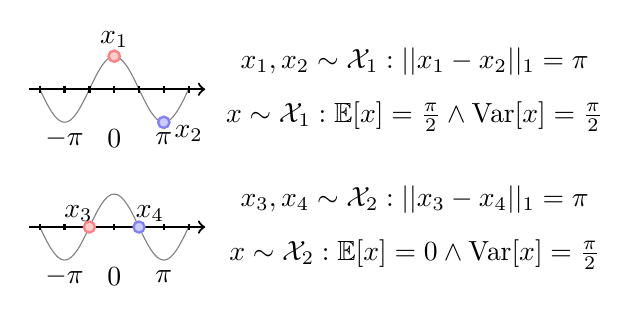
\begin{tikzpicture}
        [scale=0.7,
        inner sep=0.5mm,
        pd/.style={circle,draw=red!50,fill=red!20,thick},
        hc/.style={circle,draw=blue!50,fill=blue!20,thick}]
        
        \node (sinusoid1) at (0,0) {};
        
        \draw[black, thick, ->] ($(sinusoid1)+(-2,0.3)$) -- ($(sinusoid1)+(1.2,0.3)$);%xaxis
        \draw[thin, black!50] ($(sinusoid1)+(0.9,0.3)$) sin ($(sinusoid1)+(0.45,-0.3)$);
        \draw[thin, black!50] ($(sinusoid1)+(0.45,-0.3)$) cos ($(sinusoid1)+(0.,0.3)$);
        \draw[thin, black!50] ($(sinusoid1)+(0.,0.3)$) sin ($(sinusoid1)+(-0.45,0.9)$);
        \draw[thin, black!50] ($(sinusoid1)+(-0.45,0.9)$) cos ($(sinusoid1)+(-0.9,0.3)$);
        \draw[thin, black!50] ($(sinusoid1)+(-0.9,0.3)$) sin ($(sinusoid1)+(-1.35,-0.3)$);
        \draw[thin, black!50] ($(sinusoid1)+(-1.35,-0.3)$) cos ($(sinusoid1)+(-1.8,0.3)$);
        
        
        \draw[black, thick] ($(sinusoid1)+(-1.8,0.36)$) -- ($(sinusoid1)+(-1.8,0.24)$);
        \draw[black, thick] ($(sinusoid1)+(-1.35,0.36)$) -- ($(sinusoid1)+(-1.35,0.24)$);
        \draw[black, thick] ($(sinusoid1)+(-0.9,0.36)$) -- ($(sinusoid1)+(-0.9,0.24)$);
        \draw[black, thick] ($(sinusoid1)+(-0.45,0.36)$) -- ($(sinusoid1)+(-0.45,0.24)$);
        \draw[black, thick] ($(sinusoid1)+(0.,0.36)$) -- ($(sinusoid1)+(0.,0.24)$);
        \draw[black, thick] ($(sinusoid1)+(0.45,0.36)$) -- ($(sinusoid1)+(0.45,0.24)$);
        \draw[black, thick] ($(sinusoid1)+(0.9,0.36)$) -- ($(sinusoid1)+(0.9,0.24)$);
        
        \node at ($(sinusoid1)+(-1.35,-0.6)$) {$-\pi$};
        \node at ($(sinusoid1)+(-0.45,-0.6)$) {$0$};
        \node at ($(sinusoid1)+(0.45,-0.6)$) {$\pi$};
        
        \node (ind1) at ($(sinusoid1)+(-0.45,0.9)$) [pd] {};
        \node (ind1) at ($(sinusoid1)+(0.45,-0.3)$) [hc] {};
        
        \node (ind1) at ($(sinusoid1)+(-0.45,0.9)$) [pd] {};
        \node (ind1) at ($(sinusoid1)+(0.45,-0.3)$) [hc] {};
        
        
        \node (sinusoid2) at ($(sinusoid1)+(0,-2.5)$) {};
        
        \draw[black, thick, ->] ($(sinusoid2)+(-2,0.3)$) -- ($(sinusoid2)+(1.2,0.3)$);%xaxis
        \draw[thin, black!50] ($(sinusoid2)+(0.9,0.3)$) sin ($(sinusoid2)+(0.45,-0.3)$);
        \draw[thin, black!50] ($(sinusoid2)+(0.45,-0.3)$) cos ($(sinusoid2)+(0.,0.3)$);
        \draw[thin, black!50] ($(sinusoid2)+(0.,0.3)$) sin ($(sinusoid2)+(-0.45,0.9)$);
        \draw[thin, black!50] ($(sinusoid2)+(-0.45,0.9)$) cos ($(sinusoid2)+(-0.9,0.3)$);
        \draw[thin, black!50] ($(sinusoid2)+(-0.9,0.3)$) sin ($(sinusoid2)+(-1.35,-0.3)$);
        \draw[thin, black!50] ($(sinusoid2)+(-1.35,-0.3)$) cos ($(sinusoid2)+(-1.8,0.3)$);
        
        
        \draw[black, thick] ($(sinusoid2)+(-1.8,0.36)$) -- ($(sinusoid2)+(-1.8,0.24)$);
        \draw[black, thick] ($(sinusoid2)+(-1.35,0.36)$) -- ($(sinusoid2)+(-1.35,0.24)$);
        \draw[black, thick] ($(sinusoid2)+(-0.9,0.36)$) -- ($(sinusoid2)+(-0.9,0.24)$);
        \draw[black, thick] ($(sinusoid2)+(-0.45,0.36)$) -- ($(sinusoid2)+(-0.45,0.24)$);
        \draw[black, thick] ($(sinusoid2)+(0.,0.36)$) -- ($(sinusoid2)+(0.,0.24)$);
        \draw[black, thick] ($(sinusoid2)+(0.45,0.36)$) -- ($(sinusoid2)+(0.45,0.24)$);
        \draw[black, thick] ($(sinusoid2)+(0.9,0.36)$) -- ($(sinusoid2)+(0.9,0.24)$);
        
        \node at ($(sinusoid2)+(-1.35,-0.6)$) {$-\pi$};
        \node at ($(sinusoid2)+(-0.45,-0.6)$) {$0$};
        \node at ($(sinusoid2)+(0.45,-0.6)$) {$\pi$};
        
        \node (ind1) at ($(sinusoid2)+(-0.9,0.3)$) [pd] {};
        \node (ind1) at ($(sinusoid2)+(0.,0.3)$) [hc] {};
        
        
        \node at ($(sinusoid1)+(-0.45,1.2)$) {$x_1$};
        \node at ($(sinusoid1)+(0.9,-0.5)$) {$x_2$};
        
        \node at ($(sinusoid2)+(-1.1,0.55)$) {$x_3$};
        \node at ($(sinusoid2)+(0.2,0.55)$) {$x_4$};
        
        \node (distance1) at ($(sinusoid1)+(5,0.8)$) {$x_1, x_2 \sim \mathcal{X}_1: ||x_1-x_2||_1=\pi$};
        \node at ($(distance1)+(0,-1)$) {$x \sim \mathcal{X}_1: \mathbb{E}[x] = \frac{\pi}{2} \wedge \mbox{Var}[x]=\frac{\pi}{2}$};
        
        \node (distance2) at ($(sinusoid2)+(5,0.8)$) {$x_3, x_4 \sim \mathcal{X}_2: ||x_3-x_4||_1=\pi$};
        \node at ($(distance2)+(0,-1)$) {$x \sim \mathcal{X}_2: \mathbb{E}[x] = 0 \wedge \mbox{Var}[x]=\frac{\pi}{2}$};
    \end{tikzpicture}
    \caption{Description of how two similarly distributed samples, taken from $\mathcal{X}_1$ and $\mathcal{X}_2$, can lead to different portions of the cosine function image, since a sinusoid is periodic. Two distributions $\mathcal{X}_1$ and $\mathcal{X}_2$, may be mapped to the same image (second/bottom example). This is why a cosine is a shift invariant function. However, there are intervals a shift can be made and it is not invariant. Such intervals take the form $\forall i \in \mathbb{Z}: [i \pi, (i+1)\pi]$.}
    \label{fig:s1}
\end{figure}

\section*{S2. Separation under the random cosine projection}

\begin{proposition}[Separation under cosine projection]
Let $z_1, z_2 \in \mathbb{R}^d$ and let
\[\phi(z) = \left[\cos(\omega_1^\top z + \beta_1), \dots, \cos(\omega_d^\top z + \beta_d)\right]\]
with independent $\omega_i \sim \mathcal{N}(0, I_d)$ and $\beta_i \sim \mathrm{Uniform}[0, 2\pi]$. Then
\[
\mathbb{E}_{\omega, \beta}\left[\phi(z_1)^\top \phi(z_2)\right] = \frac{d}{2}\, e^{-\frac{1}{2}\|z_1 - z_2\|_2^2},
\]
so the expected similarity of the projected points decreases exponentially with their latent distance, and a contrastive margin that increases the latent distance between classes decreases their expected similarity after projection.
\end{proposition}

\begin{proof}[Proof of Proposition S1]
Let
\[\phi(z) = \left[ \cos(\omega_1^\top z + \beta_1), \dots, \cos(\omega_d^\top z + \beta_d) \right],\]
where each $\omega_i \sim \mathcal{N}(0, I_d)$ and $\beta_i \sim \mathrm{Uniform}[0, 2\pi]$. The inner product between projected vectors is:
\[
\phi(z_1)^\top \phi(z_2) = \sum_{i=1}^d \cos(\omega_i^\top z_1 + \beta_i) \cos(\omega_i^\top z_2 + \beta_i).
\]
Using the trigonometric identity:
\[
\cos(a)\cos(b) = \frac{1}{2}[\cos(a - b) + \cos(a + b)],
\]
we write:
\begin{align*}
    &\cos(\omega_i^\top z_1 + \beta_i) \cos(\omega_i^\top z_2 + \beta_i) = \\
&\frac{1}{2} \left[ \cos(\omega_i^\top(z_1 - z_2)) + \cos(\omega_i^\top(z_1 + z_2) + 2\beta_i) \right].    
\end{align*}


Taking the expectation over $\beta_i \sim \mathrm{Uniform}[0, 2\pi]$, the second term vanishes:
\[
\mathbb{E}_{\beta_i}[\cos(\omega_i^\top(z_1 + z_2) + 2\beta_i)] = 0.
\]

Thus,
\[
\mathbb{E}_{\omega, \beta}[\phi(z_1)^\top \phi(z_2)] = \frac{1}{2} \sum_{i=1}^d \mathbb{E}_{\omega_i}[\cos(\omega_i^\top(z_1 - z_2))].
\]

Let $\delta = z_1 - z_2$. Since $\omega_i^\top \delta \sim \mathcal{N}(0, \|\delta\|_2^2)$, we use the identity:
\[
\mathbb{E}_{x \sim \mathcal{N}(0, \sigma^2)}[\cos(x)] = e^{-\frac{1}{2}\sigma^2},
\]
to obtain:
\[
\mathbb{E}_{\omega_i}[\cos(\omega_i^\top \delta)] = e^{-\frac{1}{2}\|\delta\|_2^2}.
\]

Putting it together:
\[
\mathbb{E}_{\omega, \beta}[\phi(z_1)^\top \phi(z_2)] = \frac{d}{2} e^{-\frac{1}{2}\|z_1 - z_2\|_2^2}.
\]

which is at most $d/2$ and decreases strictly and exponentially with $\|z_1 - z_2\|_2$, proving the result.
\end{proof}

\section*{S3. Extension to more than two classes}

A multi-class solution is to consider the unitary circle in Fig.~\ref{fig:s2}. Let the pairs of data be $(x_1, x_2, y_1, y_2, y_p)$. By definition $x_1 := \mathbf{x}_2 \in \mathbb{R}^E$. And consider the targets $y_1, y_2 \in [0,1]^C$. Now $y_p$ instead of being in $[0,1]$, consider $y_p=||argmax(y_1) - argmax(y_2)||_1^1 \times \frac{\pi}{C}$ so that the possible values are $\in \{0,\frac{\pi}{C}, \dots, \frac{C\pi}{C}\}$. The contrastive loss now only needs one of its terms and can be written as
\begin{equation}\label{future_work:equation:multi_contrastive}
    \mathcal{L}_D(x_1, x_2, y_p) = ||D(x_1, x_2)-y_p||_1^1 .
\end{equation}
The other change that is needed is to apply the softmax at the output of the classifier, so that $y\in \Delta^C$.

\begin{figure}[!htbp]
    \centering
    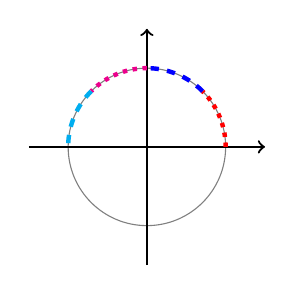
\begin{tikzpicture}
        [scale=1.,
        inner sep=0.5mm,
        pd/.style={circle,draw=red!50,fill=red!20,thick},
        hc/.style={circle,draw=blue!50,fill=blue!20,thick}]
        
        %draw unit circle
        \node (uni_circle1) at (0,0) {};
        \draw[black!50, thin] ($(uni_circle1)$) circle [radius=1];
        \draw[black, thick, ->] ($(uni_circle1)+(-1.5,0)$) -- ($(uni_circle1)+(1.5,0)$);%xaxis
        \draw[black, thick, ->] ($(uni_circle1)+(0,-1.5)$) -- ($(uni_circle1)+(0,1.5)$);%yaxis       

        \draw [dotted, ultra thick,red,domain=0:45] plot ({cos(\x)}, {sin(\x)});
        \draw [dashed, ultra thick,blue,domain=45:90] plot ({cos(\x)}, {sin(\x)});
        \draw [dotted, ultra thick,magenta,domain=90:135] plot ({cos(\x)}, {sin(\x)});
        \draw [dashed, ultra thick,cyan,domain=135:180] plot ({cos(\x)}, {sin(\x)});

        
    \end{tikzpicture}
    \caption{Hypothesis to separate multiple groups of data using the sinusoid projection. The example considers $C=4$.}
    \label{fig:s2}
\end{figure}

\end{document}
